\documentclass[10pt]{beamer}
% \documentclass[12pt]{article}
% \usepackage[noxcolor]{beamerarticle}

\usetheme[progressbar=frametitle]{metropolis}
\usepackage{appendixnumberbeamer}

\usepackage{booktabs}
\usepackage[scale=2]{ccicons}

\usepackage{pgfplots}
\usepgfplotslibrary{dateplot}

\usepackage{xspace}
\newcommand{\themename}{\textbf{\textsc{metropolis}}\xspace}

%%%%%%%% Custom Lib
\usepackage{multirow}
\usepackage{fancyvrb}
\usepackage{fancybox}
\setbeamertemplate{frame footer}{Sandeep Suman}
\usepackage[ddmmyyyy]{datetime}
\renewcommand{\dateseparator}{--}
\usepackage{tcolorbox}
\newtcolorbox{mybox}[2][]{fonttitle=\bfseries,
attach boxed title to top center={yshift=-2mm},
title=#2,#1}

\usepackage{tikz}
\usetikzlibrary{calc}
\usetikzlibrary{positioning}
\usetikzlibrary{arrows,shapes}
% \setbeamertemplate{foot{}line}[text line]{%
%   \parbox{\linewidth}{\vspace*{-8pt}Sandeep Suman\hfill\insertpagenumber}}



\title{\LaTeX}
\subtitle{Quick Start}
% \date{\today}
\date{}
\author{Sandeep Suman}
\institute{Tilka Manjhi Bhagalpur University, Bhagalpur}
% \titlegraphic{\hfill\includegraphics[height=1.5cm]{logo.pdf}}

\begin{document}

\maketitle

\begin{frame}{Table of contents}
  \setbeamertemplate{section in toc}[sections numbered]
  \tableofcontents[hideallsubsections]
\end{frame}
\tikzstyle{every picture}+=[remember picture]
\section{Introduction}
\metroset{block=fill}
\begin{frame}{History}
  \begin{description}
     \item[1982] {\TeX}  is developed by {\em Donald Knuth}\footnote{\url{https://en.wikipedia.org/wiki/Donald_Knuth}} in 1982 in order to 	type his acclaimed series of books on computer programming \emph{"Art of Computer Programming"}. 
     
     \item[1985]  Leslie Lamport extend the {\TeX} system so it will be easy to create books, article etc. This is called {\LaTeX}.
          
     \item[1993] Second edition of {\LaTeX} is launched and it is called {\LaTeX2e} which is mostly used now a days.
     
     \item[\textsc{Future}] {\LaTeX3e} is under development from long time.
     
  \end{description}
\end{frame}


\begin{frame}[fragile]{{\LaTeX ~} vs WYSIWYG}
\uncover<1->{Pros:}
    \begin{itemize}
        \uncover<2->{\item Large Document}
        \uncover<3->{\item Different types of Environment}
        \uncover<4->{\item Publication Quality}
        \uncover<5->{\item Automation}
        \uncover<6->{\item Easy to Convert to Other Format}
    \end{itemize}
  
\uncover<7->{Cons:}
	\begin{itemize}
    	\uncover<8->{\item Small Document}
        \uncover<9->{\item Difficult to Learn}
        \uncover<10->{\item \color{red}{Difficult to Edit}}
    \end{itemize}
\end{frame}  

\section{Quick Start}

\begin{frame}[fragile]{Structure\footnote{\url{https://en.wikibooks.org/wiki/LaTeX/Document_Structure}}}

\begin{center}
\textbf{Source $\Rightarrow $ Output}
\end{center}

\begin{table}[]
\centering
\label{my-label}
\begin{tabular}{lllll}
\multirow{3}{*}{Prelims} & \multirow{3}{*}{{\fontsize{30}{50}\selectfont \textbraceleft}} & \textbackslash documentclass\{...\} &  &  \\
                         &                                 & $\ldots$                            &  &  \\
\multirow{3}{*}{Content} & \multirow{3}{*}{{\fontsize{30}{60}\selectfont \textbraceleft}} & \textbackslash begin\{document\}   &  &  \\
                         &                                 & $\ldots$                  &  &  \\
                         &                                 & \textbackslash end\{document\}   &  & 
\end{tabular}
\caption{Global Structure of \LaTeX ~ Source File}
\end{table}
\end{frame}


\begin{frame}[fragile]{Document Sectioning
\footnote{\url{https://www.sharelatex.com/learn/Sections_and_chapters}}
\footnote{\url{http://www.ctex.org/documents/packages/layout/titlesec.pdf}}}
 There are up to 7 levels of depth for defining sections depending on the document class:
\begin{itemize}
\item \verb|\part{part}|
\item \verb|\chapter{chapter}|
\item \verb|\section{section}|
\item \verb|\subsection{subsection}|
\item \verb|\subsubsection{subsubsection}|
\item \verb|\paragraph{paragraph}|
\item \verb|\subparagraph{subparagraph}|
\end{itemize}

\textbf{Note:} To get a unumbered section use \verb|\section*{section}|, similarly to get an unumbered subsection use \verb|\subsection*{subsection}|.
\end{frame}

\section{Text Mode}

\begin{frame}{Font
\footnote{\url{https://en.wikibooks.org/wiki/LaTeX/Fonts}} 
\footnote{\scriptsize \url{https://www.sharelatex.com/learn/Font_sizes,_families,_and_styles}}}
  \begin{tabular}{ll}
    Regular                                                               &   Regular \\
    \textbackslash textit\{Italic\}                                       &   \textit{Italic} \\
    \textbackslash underline\{underline\}                                   &   \underline{underline}\\
    \textbackslash textsc\{SmallCaps\}                                    &   \textsc{SmallCaps} \\
    \textbackslash textbf\{Bold\}                                         &   \textbf{Bold} \\
    \textbackslash textbf\{\textbackslash textit\{ Bold Italic \}\}       &   \textbf{\textit{Bold Italic}} \\
    \textbackslash textbf\{\textbackslash textsc\{ Bold SmallCaps \}\}    &   \textbf{\textsc{Bold SmallCaps}}
   \end{tabular} 
  
%     \item[\textbackslash textbf \{ \textsc \{ Bold SmallCaps \} \} ]                  
%     \item[\textbackslash texttt \{ Monospace}]                                \texttt{Monospace}
%     \item[\textbackslash texttt \{ \textit{Monospace Italic}}]                \texttt{\textit{Monospace Italic}}
%     \item[\textbackslash texttt \{ \textbf{Monospace Bold}}]                  \texttt{\textbf{Monospace Bold}}
%     \item[\textbackslash texttt \{ \textbf{\textit{Monospace Bold Italic}}}]  \texttt{\textbf{\textit{Monospace Bold Italic}}}
\end{frame}

\begin{frame}[fragile]{Alignment
\footnote{\url{https://www.sharelatex.com/learn/Text_alignment}}}
\begin{itemize}
	\item \verb|\begin{flushleft} ... \end{flushleft}| (Default)
	\item \verb|\begin{flushright} ... \end{flushright}|
	\item \verb|\begin{center} ... \end{center}|
\end{itemize}
\pause
\begin{mybox}[]{A Right Aligned Paragraph}
\begin{flushright}
\textbf{Munger} is a twin city and a Municipal Corporation situated in the Indian state of Bihar. It is the administrative headquarters of Munger district and Munger Division.\\

\midskip Historically, Munger is known for being an ancient seat of rule. The twin city comprises Munger and Jamalpur situated on the southern bank of the river Ganges.\\
(Source: Wikipedia)
\end{flushright}
\end{mybox}
\end{frame}

\begin{frame}[fragile]{Manual breaks
\footnote{\url{https://en.wikibooks.org/wiki/LaTeX/Paragraph_Formatting\#Manual_breaks}}}
\begin{tabular}{l p{8cm}}
	\verb|\newline| 	    & Breaks the line at the point of the command.\\[1em]
	\verb|\\|	            & Breaks the line at the point of the command, it is usually a shorter version of the previous command.\\[1em]
	\verb|\\*|              & Breaks the line at the point of the command and also prohibits a page break after the forced line break. \\[1em]
	\verb|\\[extra-space]|  & Extra vertical space to be inserted before the next line. This amount can be negative.\\[1em]
	\verb|\par| (TeX)       & Starts a new paragraph. \\[1em]
	\verb|\newpage|         & Starts a new page.
\end{tabular}	
\end{frame}


\begin{frame}[fragile]{Lists}  
  \begin{columns}[T,onlytextwidth]
  
    \column{0.33\textwidth}
		\underline{Unordered List}
        
\begin{verbatim}
\begin{itemize}
  \item Milk 
  \item Eggs 
  \item Potatoes
\end{itemize}\end{verbatim}
      
      \begin{itemize}
      \item Milk \item Eggs \item Potatoes
      \end{itemize}
      
    \column{0.33\textwidth}
    \underline{Enumerations}
    
\begin{verbatim}
\begin{enumerate}
  \item First 
  \item Second
  \item Last
\end{enumerate}\end{verbatim}

    \begin{enumerate}
    \item First \item Second \item Last
    \end{enumerate}

    \column{0.33\textwidth}
    \underline{Description}
    \begin{verbatim}
\begin{description}
  \item[Ram] One 
  \item[Shyam] Two
  \item[Mohan] Three
\end{description}\end{verbatim}

    \begin{description}
      \item[Ram] One 
      \item[Shyam] Two
      \item[Mohan] Three
    \end{description}
\end{columns}
\pause
\begin{tikzpicture}[overlay]
\draw[red, rounded corners=2ex] (0.2,4.2)rectangle (3.2,2.75);
\draw[red, rounded corners=2ex] (3.8,4.2)rectangle (6.4,2.75);
\end{tikzpicture}
\end{frame}

\begin{frame}[fragile]{Tables
\footnote{\url{https://en.wikibooks.org/wiki/LaTeX/Tables}}
\footnote{\url{https://www.sharelatex.com/learn/Tables}}}

\begin{columns}[T,onlytextwidth]
\column{0.5\textwidth}
\vspace{-0.5cm}
\begin{verbatim}
 \begin{tabular}{ l c r }
  a   & a   & a   \\
  ab  & ab  & ab  \\ 
  abc & abc & abc \\ 
\end{tabular}
\end{verbatim}
\vspace{0.5cm}
 \begin{tabular}{ l c r }
  a   & a   & a   \\
  ab  & ab  & ab  \\ 
  abc & abc & abc \\ 
\end{tabular}


\column{0.5\textwidth}
\vspace{-0.5cm}
\begin{verbatim}
\begin{tabular}{ l | c r |}
  a   & a   & a   \\ \hline
  ab  & ab  & ab  \\ 
  abc & abc & abc \\ 
\end{tabular}
\end{verbatim}
\vspace{0.5cm}
\begin{tabular}{ l | c r |}
  a   & a   & a   \\ \hline
  ab  & ab  & ab  \\ 
  abc & abc & abc \\ 
\end{tabular}
\end{columns}

\end{frame}

\begin{frame}[fragile]{Floating with Table
\footnote{\url{https://en.wikibooks.org/wiki/LaTeX/Tables\#Floating_with_table}}}
\begin{table}
\begin{tabular}{l p{10cm}}
h & where the table is declared (here)\\[1em]
t & at the top of the page\\[1em]
b & at the bottom of the page\\[1em]
p & on a dedicated page of floats\\[1em]
! & override the default float restrictions. E.g., the maximum size allowed of a b float is normally quite small; if you want a large one, you need this ! parameter as well.
\end{tabular}
\end{table}
\textbf{Note:} Default is {\color{blue} \texttt{tbp}}. If you want a table at the position it is specified, you should use \ovalbox{\texttt{h!}}.
\end{frame}

\begin{frame}[fragile]{Pictures
\footnote{\url{https://www.sharelatex.com/learn/Inserting_Images}}
\footnote{\url{https://en.wikibooks.org/wiki/LaTeX/Importing_Graphics}}}

To include a figure in {\LaTeX } we have to use \textbf{graphicx} package, and a figure in \texttt{.eps}, \texttt{.png} or \texttt{.pdf} format is added using \verb|\includegrapics|. Some uses are as follows:
\begin{itemize}
\item \verb|\includegraphics{filename}|   Simple Use \pause
\item \verb|\includegraphics[scale=1.5]{filename}| Scale the figure by factor of $1.5$ \pause
\item \verb|\includegraphics[width=3cm, height=4cm]{filename}| Specific height and width of figure \pause
\item \verb|\includegraphics[width=\textwidth]{universe}| Width same as document
\end{itemize}
\end{frame}

\begin{frame}[fragile]{Example}

\begin{verbatim}
      \begin{figure}[h]
       \centering
       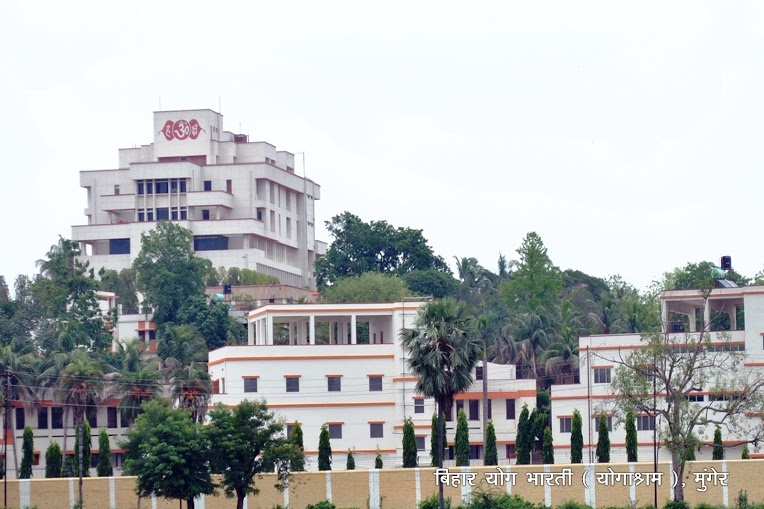
\includegraphics[height=3cm]{images/munger-pic}
       \caption{A picture of munger}
      \end{figure}
\end{verbatim}

\begin{figure}[h]
 \centering
 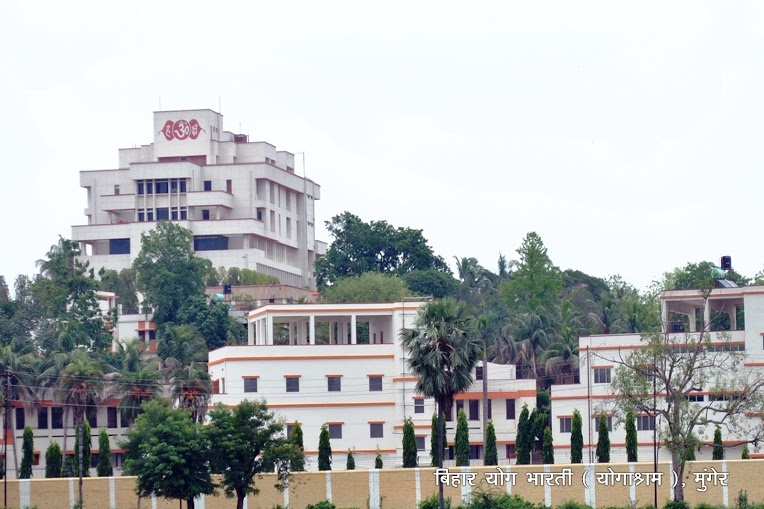
\includegraphics[height=2cm]{images/munger-pic}
 \caption{A picture of munger}
\end{figure}

\end{frame}

\begin{frame}{Example -- Line plots}
  \begin{figure}
    \begin{tikzpicture}
      \begin{axis}[
        mlineplot,
        width=0.9\textwidth,
        height=6cm,
      ]

        \addplot {sin(deg(x))};
        \addplot+[samples=100] {sin(deg(2*x))};

      \end{axis}
    \end{tikzpicture}
  \end{figure}
\end{frame}

\begin{frame}{Example -- Bar charts}
  \begin{figure}
    \begin{tikzpicture}
      \begin{axis}[
        mbarplot,
        xlabel={Foo},
        ylabel={Bar},
        width=0.9\textwidth,
        height=6cm,
      ]

      \addplot plot coordinates {(1, 20) (2, 25) (3, 22.4) (4, 12.4)};
      \addplot plot coordinates {(1, 18) (2, 24) (3, 23.5) (4, 13.2)};
      \addplot plot coordinates {(1, 10) (2, 19) (3, 25) (4, 15.2)};

      \legend{lorem, ipsum, dolor}

      \end{axis}
    \end{tikzpicture}
  \end{figure}
\end{frame}

\begin{frame}[fragile]{Quotes }
\begin{verbatim}
 \begin{quote}
   Young man, in mathematics you don't understand things. 
   You just get used to them.\\
   \hfill --- \textup{John Von Neumann}
 \end{quote}
\end{verbatim}
 
 \vskip1cm

\begin{quote}
Young man, in mathematics you don't understand things. You just get used to them.\\
\hfill --- \textup{John Von Neumann}
\end{quote}
\end{frame}

\begin{frame}[fragile]{Quotation }
\begin{verbatim}
 \begin{quotation}
   Young man, in mathematics you don't understand things. 
   You just get used to them.\\
   \hfill --- \textup{John Von Neumann}
 \end{quotation}
\end{verbatim}
 
 \vskip1cm

\begin{quotation}
Young man, in mathematics you don't understand things. You just get used to them.\\
\hfill --- \textup{John Von Neumann}
\end{quotation}
\end{frame}

\section{Math Mode}


\begin{frame}{Mathematical Expression
\footnote{\url{http://reu.dimacs.rutgers.edu/Symbols.pdf}}   			   
\footnote{\url{https://en.wikibooks.org/wiki/LaTeX/Mathematics}}
\footnote{\url{https://www.sharelatex.com/learn/Mathematical_expressions}}
\footnote{\url{http://www.math.hkbu.edu.hk/TeX/short-math-guide.pdf}}
}
	\begin{itemize}
    	\uncover<1->{\item Inline Expression
        	\begin{itemize}
            	\item \$ $\ldots$ \$ or \textbackslash ( $\ldots$ \textbackslash )  
                \item Mixed with text.
            \end{itemize}}
            
        \uncover<2->{\item Display Style    
        	\begin{itemize}
            	\item Untagged: \$\$ $\ldots $ \$\$ or \textbackslash [ $\ldots $ \textbackslash ] 
                \item Tagged: \textbackslash begin\{ equation\} $\ldots$ \textbackslash end\{ equation\}
            \end{itemize}}
            
        \uncover<3->{\item A Set of Equation
        	\begin{itemize}
            	\item \AmS-\LaTeX: align, aligned
            	\item \texttt{mathtools}: gather
            	\item \textsf{equarray}: eqnarray
            \end{itemize}}            
        
    \end{itemize}
\end{frame}




\begin{frame}[fragile]{Example}
\begin{verbatim}This is an inline equation \(x^2 + y^2 = z^2\).The following 
equation is in "Display Style".

\[ x^n + y^n = z^n \]

The following equation is numbered.
\begin{equation} x^n + y^n = z^n \end{equation}\end{verbatim}
  \begin{center}$\Downarrow $\end{center}
This is an inline equation \(x^2 + y^2 = z^2\).
The following equation is in "Display Style".
\[ x^n + y^n = z^n \]
The following equation is numbered.
\begin{equation}
 x^n + y^n = z^n
\end{equation}
\end{frame}

\begin{frame}[fragile]{Example - Set of Equation}

\begin{verbatim}\begin{align*}
 f(x)  &= a x^2+b x +c   &   g(x)  &= d x^3 \\
 f'(x) &= 2 a x +b       &   g'(x) &= 3 d x^2
\end{align*}\end{verbatim}
\pause
  $$\Downarrow $$
\begin{align*}
 f(x)  &= a x^2+b x +c   &   g(x)  &= d x^3 \\
 f'(x) &= 2 a x +b       &   g'(x) &= 3 d x^2
\end{align*}
\end{frame}


\begin{frame}[fragile]{Matrices }
Although matrices can be print using tabular enviroment. But there are some predefined matrices in \AmS-\LaTeX.

\begin{verbatim}
                       \begin{pmatrix}
                        a & b \\ 
                        c & d 
                       \end{pmatrix}
\end{verbatim}

$$\begin{pmatrix}a & b \\ c & d \end{pmatrix}$$
\end{frame}
\begin{frame}[fragile]{Matrices }
Although matrices can be print using tabular enviroment. But there are some predefined matrices in \AmS-\LaTeX.
\begin{verbatim}
                       \begin{bmatrix}
                        a & b \\ 
                        c & d 
                       \end{bmatrix}
\end{verbatim}

$$\begin{bmatrix}a & b \\ c & d \end{bmatrix}$$
\end{frame}
\begin{frame}[fragile]{Matrices }
Although matrices can be print using tabular enviroment. But there are some predefined matrices in \AmS-\LaTeX.
\begin{verbatim}
                       \begin{vmatrix}
                        a & b \\ 
                        c & d 
                       \end{vmatrix}
\end{verbatim}  

$$\begin{vmatrix}a & b \\ c & d \end{vmatrix}$$
\end{frame}
\begin{frame}[fragile]{Matrices }
Although matrices can be print using tabular enviroment. But there are some predefined matrices in \AmS-\LaTeX.

\begin{verbatim}
                       \begin{Vmatrix}
                        a & b \\ 
                        c & d 
                       \end{Vmatrix}
\end{verbatim}

$$\begin{Vmatrix}a & b \\ c & d \end{Vmatrix}$$

\end{frame}



\begin{frame}[fragile]{Cases}

\begin{verbatim}
     f(x) = 
       \begin{cases} 
        1       & \text{if } x \in \mathbb{Q} \\
        0       & \text{else }  
       \end{cases}
\end{verbatim}

$$\Downarrow $$
\vspace{0.5cm}
$$ f(x) = 
  \begin{cases} 
   1       & \text{if } x \in \mathbb{Q} \\
   0       & \text{if } \text{else} 
  \end{cases}$$

\end{frame}

\section{Advance Mathematics}

\begin{frame}[fragile]{Custom Operator}
\begin{tcolorbox}[width=\textwidth, colframe=red]
A custom operator like $\sin(x)$, use \verb|\DeclareMathOperator| command in preamble or 
\verb|\operatorname| in document itself. 
\end{tcolorbox}

\begin{tabular}{ll}
\verb|\operatorname{E}[x]|             & $E[X] = \operatorname{E}[X]$ \\[1em]
\verb|\operatorname{arg\,max}_a f(a)|  & $\operatorname{arg\,max}_a f(a)$ \\[1em]
\end{tabular}

\begin{tcolorbox}[width=\textwidth, colframe=red]
To get a operator like \verb|\lim|, either use \verb|\DeclareMathOperator*| or \verb|\operatorname*|
commnad, for example
\end{tcolorbox}

\begin{verbatim}
  \operatorname{foo}_a f(a) = \operatorname*{foo}_b f(b)
\end{verbatim}
$$\operatorname{foo}_a f(a) = \operatorname*{foo}_b f(b)$$
\end{frame}

\begin{frame}[fragile]{Whitespace in Math Mode}
\begin{tabular}{ll}
\verb|\quad| &	space equal to the current font size (= 18 mu) \\[1em]
\verb|\,|    &	3/18 of \verb|\quad| (= 3 mu)\\[1em]
\verb|\:|    &	4/18 of \verb|\quad| (= 4 mu)\\[1em]
\verb|\;|	 &  5/18 of \verb|\quad| (= 5 mu)\\[1em]
\verb|\!| 	 &  -3/18 of \verb|\quad| (= -3 mu)\\[1em]
\verb|\ |    &	equivalent of space in normal text\\[1em]
\verb|\qquad|&	twice of \verb|\quad| (= 36 mu)
\end{tabular}
\end{frame}

\begin{frame}[fragile]{Whitespace - Phantom}
\begin{tcolorbox}[width=\textwidth, colframe=red]
Another way to make whitespace is to make somthing invisible. We can use \verb|\phantom| command to make something invisible in math mode.
\end{tcolorbox}
\begin{verbatim}
\begin{pmatrix} -1 & -2\\ 2 & 1 \end{pmatrix} = 
\begin{pmatrix} -1 & -2\\ \phantom{-}2 & \phantom{-}1
\end{pmatrix}
\end{verbatim}
$$\begin{pmatrix} -1 & -2 \\ 2 & 1 \end{pmatrix} = \begin{pmatrix} -1 & -2 \\ \phantom{-}2 & \phantom{-}1\end{pmatrix}$$
\end{frame}

\begin{frame}[fragile]{Left and Right Delimiter}
\begin{tcolorbox}[width=\textwidth, colframe=red]
Proper size of paranthesis is obtained using \verb|\left| and \verb|\right| delimeter
\end{tcolorbox}
\begin{verbatim}
\{ 
\begin{pmatrix} 1 \\ n \end{pmatrix} | n \in \mathbb{N} 
\} = \left \{ 
\begin{pmatrix} 1 \\ n \end{pmatrix} | n \in \mathbb{N} 
\right \}
\end{verbatim}
$$\{ \begin{pmatrix} 1 \\ n \end{pmatrix} | n \in \mathbb{N} \} = \left \{ 
\begin{pmatrix} 1 \\ n \end{pmatrix} | n \in \mathbb{N} 
\right \}$$
\end{frame}

\section{More to Explore}

\begin{frame}
\begin{itemize}
	\item custom command
	\item hyperref
	\item bililiography
	\item index
	\item beamer
	\item etc.
\end{itemize}
\end{frame}

{\setbeamercolor{palette primary}{fg=black, bg=orange}
\begin{frame}[standout]
  Questions?
\end{frame}
}

{\setbeamercolor{palette primary}{fg=black, bg=yellow}
\begin{frame}[standout]
  Thank You?
\end{frame}
}

\appendix

\begin{frame}{Download}

  This slide is created using beamer with metropolis theme. Last update on {\today } is avilable for download.

 \begin{center} 
 \href{https://goo.gl/jDsT79}{\color{blue}{\Ovalbox{\large\bf Download}}}
 \end{center}

  The Slide is licensed under a
  \href{http://creativecommons.org/licenses/by-sa/4.0/}{Creative Commons
  Attribution-ShareAlike 4.0 International License}.

  \begin{center}\ccbysa\end{center}

\end{frame}

%\appendix

% \begin{frame}[fragile]{Backup slides}
%   Sometimes, it is useful to add slides at the end of your presentation to
%   refer to during audience questions.

%   The best way to do this is to include the \verb|appendixnumberbeamer|
%   package in your preamble and call \verb|\appendix| before your backup slides.

%   \themename will automatically turn off slide numbering and progress bars for
%   slides in the appendix.
% \end{frame}

% \begin{frame}[allowframebreaks]{References}

%   \bibliography{demo}
%   \bibliographystyle{abbrv}
  
  

% \end{frame}

\end{document}
